\documentclass[]{article}

\usepackage{graphicx}
\usepackage[margin=2cm]{geometry}
\usepackage[ddmmyyyy]{datetime}
\usepackage{fancyhdr}
\usepackage{appendix}
\usepackage{tabulary}
\usepackage{rotating}
\usepackage[style=ieee,backend=bibtex]{biblatex}
\usepackage{hyperref}
\usepackage{booktabs}
\usepackage{float}
\usepackage[tight]{shorttoc}
\usepackage[color=yellow]{todonotes}

\bibliography{refs}

\newcommand{\ID}{CP-CBU-155}

\let\Contentsline\contentsline
\renewcommand\contentsline[3]{\Contentsline{#1}{#2}{}}

\pagestyle{fancy}
\fancyhf{}
\lhead{\thepage}
\rhead{\textbf{\ID}}

%opening
\title{Capstone Project
	  \vfill
	Final Report
	\vfill
	2015}
\author{}
\date{}


\begin{document}
	
\begin{titlepage}
	\begin{figure}
		\centering
		
\includegraphics[width=100pt]{Images/emblem}
		\label{fig:emblem}
	\end{figure}
\end{titlepage}

\maketitle

\begin{tabular}{ll}
	Project Title: & Hybrid UAV Development for Emergency Response \\ 
	\\
	Date: & \date{\today} \\ 
\end{tabular}
\\
\\

\textbf{\textit{Project Team Information}}
\\
\\

\begin{tabular}{ll}
	Identifier: & \textbf{\ID} \\\\
	Student workers: & \begin{tabular}[t]{@{}ll}
		Matthew De Bono & 390758 \\ 
		Alexander Daraio & 389844 \\ 
		Wesley Lim & 391053 \\ 
		Shanon Loveridge & 218041 \\ 
	\end{tabular}  \\\\
	Academic supervisor: & Colin Burvill \\\\ 
	Academic examiner: & Saman Halgamuge\\\\
	Industry Mentor: & Jonathon Manton, DEEE\\\\
	Version: & 1.0 \\\\
\end{tabular} 

\vfill
\vfill

\newpage

\section*{Acknowledgements}
Team CP-CBU-155 would like to acknowledge several contributions to the project:

Melbourne School of Engineering for providing the workspace to complete the project, Colin Burvill and Saman Halgamuge for their guidance and supervision, Andrew Nolan and Jeff Hollingworth for their expertise and equipment, and the Phoenix Multicoptor teams for the laughs, advice and co-operation throughout the year.

\todomessage{Make sure to uncomment line here to generate Table of Contents, then comment out again}
\tableofcontents

\begingroup

% Modify ToC item separation
\makeatletter
\renewcommand\@dotsep{10000}
\patchcmd{\l@section}{%
	\addvspace{1.0em \@plus\p@}% original code line
}{%
	\addvspace{0.5em \@plus 0.3\p@}% substitute code line
}{}{}
\makeatother

% Generate ToC in document
%\shorttoc{Contents}{2}
\endgroup

\newpage
\section{Executive Summary}
The Executive Summary offers a succinct statement of your findings and contributions.

It will summarise the project description and your contributions to the associated discipline.  

This section can be based on key sentences and paragraphs from your Scope of Works and Progress Report documents, and your Conclusions and Recommendations section.

No more than five pages of text and images.


\subsection{Test}

\section{Introduction}
\subsection{Context}
\todo[inline]{Get references}
Drones, or UAVs, are not new technologies. UAVs are currently used extensively, for both offensive and defensive operations, by militaries across the globe. There is also a strong push for UAVs in commercial applications, such as package delivery and crop monitoring, and an ever-growing population of hobbyists, adventurers and athletes using drone-mounted cameras to capture everything from weddings to skiing down mountains.\\

\todo[inline]{Add more negatives/problems}
However, there are several applications that are infeasible for current drone technology. Rotor-based aircraft like the DJI Phantom (Figure \ref{fig:lidar}) are highly maneuverable, easy to control, and can be launched from almost any location, but as a result of their large power demands have very limited range/endurance. This makes them difficult to use in applications requiring long distance travel, such as package delivery.

\begin{figure}[!h]
	\centering
	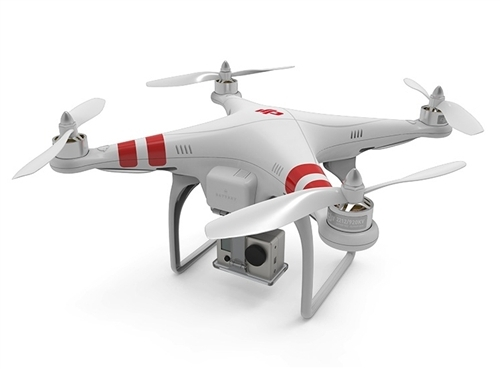
\includegraphics[width=150pt]{\IMAGEPATH /Aircraft/djiPhantom}
	\caption{DJI Phantom, a commercially available UAV}
	\label{fig:dji}
\end{figure}

\todo[inline]{Add more negatives/problems}
Wing-based aircraft such as those based on the Skywalker X8 frame (Figure \ref{fig:x8}) can achieve much greater travel distances as a result of higher efficiency flight. However, winged aircraft require open spaces to land safely, making them difficult to use in cramped or obstacle-rich applications such as low-altitude search near cities or forests.

\begin{figure}[!h]
	\centering
	
\includegraphics[width=160pt]{\IMAGEPATH /Aircraft/x8}
	\caption{Skywalker X8 airframe, a common hobby starter}
	\label{fig:x8}
\end{figure}
 
The UAV Challenge is a competition organised by the Queensland University of Technology and the CSIRO. It is held every 2 years, and aims to push the boundaries of current autonomous aircraft technology. The 2016 challenge is titled ``Medical Express'', and seeks to overcome some of the issues raised above. The objectives of the 2016 Challenge are to use unmanned aircraft to assist in a medical emergency.\\

Competitors must develop an aircraft than can fly to a known location (up to 30km) through specific transit corridors, search for and correctly identify ``Outback Joe'', land close to him to accept a pre-prepared blood sample, and then fly back to base. All of these actions must be completed within an hour, and must be autonomous; that is, after receiving the ``start'' signal the aircraft must have no human input.\\

\todo[inline]{Not sure if this section fits in intro}
The time period of the competition extends from registration (before 2nd September, 2015) to final competition (week starting 19th of September, 2016), spanning over 1 year. Table \ref{tab:challenge} highlights the key dates and corresponding stages of the UAV Challenge.\\

\todo[inline]{Add completed to D1 once we get the response}
\begin{table}[!ht]
	\caption{UAV Challenge Timeline}
	\label{tab:challenge}
	\centering
	\begin{tabular}{ | l | l | }
		\hline
		\textbf{Events} & \textbf{Date} \\ \hline \hline
		Registration and Deliverable 1: Short Technical Report & 2nd September 2015 \\ \hline
		Deliverable 2: Technical Report and Video & 13th April 2016 \\ \hline
		Deliverable 3: Autonomous Flight Record & 3rd August 2016 \\ \hline
		Final ``Go/No-Go'' decision for teams & 10th August 2016 \\ \hline
		Medical Express Challenge & Week starting 19th September 2016 \\
		\hline
	\end{tabular}
\end{table}

\subsection{\ID Contributions}
This project involves the development of an autonomous Unmanned Aerial Vehicle (UAV) with the capabilities to compete in the 2016 UAV Challenge. From the task specified above, \ID have identified a number of design and performance requirements necessary for an aircraft to be successful in the Challenge:
\begin{enumerate}[label=\bfseries R\arabic*:] \itemsep-2pt
	\item Capacity to switch between automated and manual flight modes through user commands
	\item Payload receipt and transportation back to base
	\item Take-off and landing in obstacle-rich environments (i.e. without runway)
	\item Total flight travel distance of at least 60km
	\item Total flight duration of at least 60 minutes
	\item Automated in-flight identification of a target
\end{enumerate}

\todo[inline]{Might remove some of these in final}
Given the requirements and the timeline of the Challenge above, \ID sought to develop a working prototype with which to enter the 2016 UAV Challenge. As such, the following objectives were selected for the project:
\begin{enumerate}[label=\bfseries O\arabic*:] \itemsep-2pt
	\item Register for the 2016 UAV Challenge
	\item Provide a Bill of Materials for UAV development
	\item Development of a novel hybrid flight system, incorporating both Vertical Take-Off and Landing (VTOL) and Fixed-Wing flight modes, to achieve \textbf{R3}, \textbf{R4} and \textbf{R5}
	\item Development, documentation and implementation of autonomous flight controls
	\item Development of a low-cost, medium-range sensor system to enable object detection and path planning
	\item Development of in-flight search and obstacle avoidance mechanisms to achieve \textbf{R6}
	\item Establish a strong foundation for Capstone student teams to continue work in 2016
\end{enumerate}

The remaining sections of the report will discuss the work conducted by \ID in developing a working prototype for the UAV Challenge, beginning with formulating design requirements and constraints from the UAV Challenge specification. The following sections will discuss the various domains of the aircraft, including design, flight and planning systems, and sensing systems, with a particular focus on the novel transition system for hybrid flight. The report will end with conclusions and recommendations for future work.

\section{Literature Review}
\subsection{Mission Breakdown}
\label{sec:flightmaneuvers}
The Medical Express mission can be broken down into three discrete flight maneuvers:
\begin{enumerate}[label=\bfseries M\arabic*:] \itemsep-2pt
	\item Hover flight, including vertical take-off to cruising height, and landing
	\item Fixed-wing flight, navigating through waypoints and keeping within GeoFence boundaries
	\item Aerial search
\end{enumerate}

Using these maneuvers, completing the mission can be described as completing the sequence of actions\\
\begin{tabular}{r l l}
	1. & Mission start after being armed & (\textbf{M1}) \\ 
	2. & Navigate to Joe's location & (\textbf{M2}) \\ 
	3. & Aerial search to identify Joe & (\textbf{M3}) \\ 
	4. & Land near Joe to collect blood & (\textbf{M1}) \\ 
	5. & Take-off after being re-armed & (\textbf{M1}) \\ 
	6. & Navigate back to base & (\textbf{M2}) \\ 
	7. & Land at base & (\textbf{M1}) \\ 
\end{tabular}\\

Executing this mission on a purely fixed-wing or rotor-based aircraft is unlikely to be successful; instead, teams will need to design an aircraft that makes use of both flight modes. Analysis of the 2014 design, a purely fixed-wing aircraft, showed that converting it to a hybrid aircraft would not result in a suitable design for the Challenge. Given the aircraft's weight, adding the necessary equipment would add over 5kg, cost over \$500, and would result in less than 60 seconds of flight time. It was therefore decided the 2014 model would not be suitable for the 2016 competition; a detailed analysis can be found in Appendix \ref{sec:lastYear}.\\

As this project involves the development of a novel aircraft platform, there is a lack of academic literature that is relevant to the problem at hand. This review will instead collate examples of commercial and hobby systems that were used to inspire and guide the development of the aircraft.\\

\subsection{Aircraft Design}
\subsubsection*{Arcturus Jump}
The Arcturus Jump\cite{ref:arcturus} (Figure \ref{fig:arcturus}) is a quad-copter/fixed-wing hybrid, with propellers mounted across the wings for VTOL, and a propeller at the front for fixed-wing flight. Modifying an existing airframe to emulate this design would be straightforward, but the addition of the support structure for VTOL flight would add significant weight to the aircraft, decreasing thrust and maneuverability, and increasing drag. These factors make an aircraft of this design unlikely to achieve \textbf{R4} (60km endurance) and \textbf{R5} (60min of flight) of the UAV Challenge.

\begin{figure}[!h]
	\centering
	\includegraphics[width=150pt]{\IMAGEPATH /Aircraft/arcturus}
	\caption{Arcturus Jump 20}
	\label{fig:arcturus}
\end{figure}

\subsubsection*{X PlusOne}
The X PlusOne\cite{ref:xplusone} (Figure \ref{fig:xplusone}) is an incredibly fast and efficient hybrid with four front-facing propellers. It is extremely small and light, and would be relatively cheap to build, but is too small to replicate with an existing airframe. However, based on the activities of the 2014 UAV team, designing a completely new airframe would take a significant amount of time, and is not advised for this project.

\begin{figure}[!ht]
	\centering
	\includegraphics[width=120pt]{\IMAGEPATH /Aircraft/xplusone}
	\caption{X PlusOne}
	\label{fig:xplusone}
\end{figure}

\subsubsection*{TBS Caipirinha}
The TBS Caipirinha\cite{ref:caipirinha} (Figure \ref{fig:caipirinha}) is traditionally a hobbyist fixed-wing aircraft kit. However, several examples have shown it is possible to modify the Caipirinha to be a VTOL aircraft\cite{ref:caipirinhaVTOL} (Figure \ref{fig:caipirinhaVTOL}), with two front-facing propellers. Modifying the Caipirinha for hybrid flight would require minimal modifications to the airframe but would require the development of advanced control systems to alternate between VTOL and fixed-wing modes.

\begin{figure}[!ht]
	\centering
	\begin{minipage}{.5\textwidth}
		\centering
		\includegraphics[width=135pt]{\IMAGEPATH /Aircraft/caipirinha}
		\caption{TBS Caipirinha}
		\label{fig:caipirinha}
	\end{minipage}%
	\begin{minipage}{.5\textwidth}
		\centering
		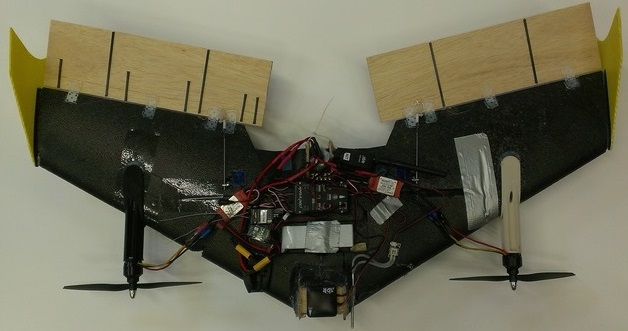
\includegraphics[width=155pt]{\IMAGEPATH /Aircraft/caipirinhaVTOL}
		\caption{Caipirinha modified for VTOL flight}
		\label{fig:caipirinhaVTOL}
	\end{minipage}
\end{figure}

\subsubsection*{Aerosense AS-DT01-E}
The Aerosense AS-DT01-E\cite{ref:sony} (Figure \ref{fig:sony}) is an autonomous hybrid VTOL/fixed-wing aircraft being developed by Sony Mobile in partnership with Japanese company ZMP. While the prototype aircraft would be an ideal candidate for the Challenge, as with the X PlusOne the design and construction of the airframe would be time consuming, and is not advised for this project.

\begin{figure}[!ht]
	\centering
	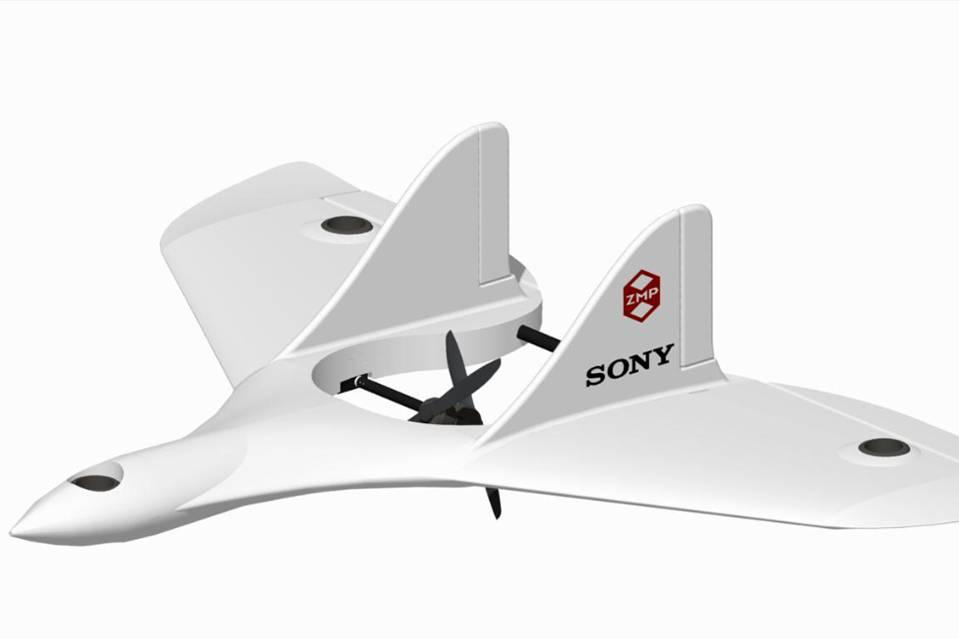
\includegraphics[width=160pt]{\IMAGEPATH /Aircraft/sony}
	\caption{Sony Aerosense}
	\label{fig:sony}
\end{figure}

\subsubsection*{FireFLY6}
Finally, the FireFLY6\cite{ref:firefly6} (Figure \ref{fig:firefly6}) is a remote control hybrid VTOL/fixed-wing aircraft consisting of six propellers arranged in 3 sets of two (Y6 configuration). This design can achieve 20-30 minutes of flight time, seven minutes of hover, and a cruising speed of 54km/h, and would be a strong contender in the UAV Challenge.

\begin{figure}[!h]
	\centering
	\includegraphics[width=160pt]{\IMAGEPATH /Aircraft/firefly6}
	\caption{FireFLY6}
	\label{fig:firefly6}
\end{figure}

\section{Summary of UAV Challenge}
The UAV Challenge is a competition held every 2 years where teams enter their UAV for the purpose of completing a autonomously search and rescuse type task.
This iteration of the challenge is titled ``Medical Express 2016'', whereby teams are tasked with using an unmanned aircraft to fly out to a known area through specific transit corridors, search and correctly identify ``Outback Joe'', land close to him, have Joe place his simulated blood sample within the aircraft and then have the aircraft fly back to base such that his blood sample can be analysed.\\

The time period of the competition extends from registration (before 2nd September, 2015) to final competition (week starting 19th of September, 2016), spanning over 1 year. The following table highlights the key dates and corresponding events of the 2016 UAV Challenge.\\

\todo[inline]{Add completed to D1 once we get the response}
\begin{center}
	\begin{tabular}{ | l | l | }
	\hline
	Events & Date \\ \hline \hline
	Registration and Deliverable 1: Short Technical Report & 2nd September 2015 \\ \hline
	Deliverable 2: Technical Report and Video & 13th April 2016 \\ \hline
	Deliverable 3: Autonomous Flight Record & 3 August 2016 \\ \hline
	Final ``Go/No-Go'' decision for teams & 10 August 2016 \\ \hline
	Medical Express Challenge & Week starting 19th September 2016 \\
	\hline
	\end{tabular}
\end{center}

\section{Formulation of Design Requirements and Constraints}
The design requirements and constraints of the project are determined by following the performance, deadline and safety requirements of the 2016 UAV Challenge, and also self-imposed constraints and requirements. For this task the required flight time, distance and maximum weight for a classification were selected as the starting parameters for the calculations.\\

Secondary objectives included the prioritization of low cost development, as well as use of readily available components and materials. The ranking of the priority of objectives is define as follows:

\begin{itemize}
	\item \textbf{High Priority:} Primary objective of the project.
	\item \textbf{Medium Priority:} Objectives that result in performance specifications (treated negotiable).
	\item \textbf{Low Priority:} Not of primary concern, but to be addressed where feasible.
	\item \textbf{Competition Priority:} Important objectives to compete in competition, but out of this years scope.
\end{itemize}

\begin{table}[!ht]
	\caption{Project Objectives for \ID}
	\label{tab:objectives}
	\begin{tabular}{ | l | c | c | }
		\hline
		\multicolumn{1}{| c |}{\textbf{Objective}} & \textbf{Criteria} & \textbf{Priority} \\
		\hline
		\multicolumn{3}{| l |}{\textbf{Compete in UAV Challenge 2016}} \\
		\hline
		Register in UAV Outback Competition & Pass/Fail & High \\
		\hline
		Submit and Pass UAV Challenge Deliverable 1 & Pass/Fail & High \\
		\hline
		\multicolumn{3}{ | c | }{ \textbf{Achieve a functional UAV}} \\
		\hline
		Achieve maiden flight & Pass/Fail & High \\
		\hline
		Achieve autonomous flight & Pass/Fail & High \\
		\hline
		\multicolumn{3}{ | c | }{ \textbf{Adhere to UAV Challenge 2016 rules}} \\
		\hline
		Be able to take off and land in obstacle rich environment & Pass/Fail & High \\
		\hline
		\multicolumn{3}{ | c | }{ \textbf{Introduce design novelty}} \\
		\hline
		Introduce transition system between VTOL and fixed-wing modes & Pass/Fail & High \\
		\hline
		Utilize 3D printed components & Pass/Fail & High \\
		\hline
		\multicolumn{3}{ | c | }{ \textbf{Adhere to UAV Challenge 2016 rules}} \\
		\hline
		Ability to take off and land in an obstacle rich environment & Pass/Fail & High \\
		\hline
		Ability to travel at least 60 kilometers & Pass/Fail & High \\
		\hline
		Ability to complete competition in at most 60 minutes & Pass/Fail & Competition \\
		\hline
		\multicolumn{3}{ | c | }{ \textbf{Other}} \\
		\hline
		Manufacturable with available resources & Pass/Fail & Low\\
		\hline
		Manufacturable with readily available components & Pass/Fail & Low\\
		\hline
		Low cost project & Total Expediture (AUD) & Low\\
		\hline
		UAV transportable via car & Pass/Fail & Low\\
		\hline
	\end{tabular}
\end{table}

The formulation of objectives, requirements and constraints provide the performance specificiations that are used as a foundation for the selection of motor, propellor and battery components.
\color{red}
Everything required, and what we have covered this year (wes,matt,shanon,alex)
\color{black}

\section{Remaining Sections}
You are welcome to choose appropriate names for section headings.

The main argument will begin with a section describing your team’s major activities, leading to the fulfilment of the objectives of your project.  A flow chart will provide a useful visual aid.

Introduce the tasks that you were required to complete to satisfy the agreed project scope.  Itemise tasks whenever possible to assist cross-referencing with following sections (i.e. your contributions).

Describe the development your ideas and strategies, the conceptual design and research methods used (as applicable), and why they were chosen (your literature review will be of value here).  

Discuss any original contributions including, for example, modifications or extensions of published methods or associated knowledge.  Your team may have made a more humble, but still valuable, contribution, where you customised an existing method for your specific application.  Describe the benefits and, if applicable, deficiencies associated with your contributions.

The criteria against which preferred concepts are identified should be discussed.  This aspect of your report, appropriately sectioned, will make extensive use of pictorial information (figures) and organised information (lists and tables).  

Given Final Report submissions are normally not paper-based, all supporting material (figures, tables) in the main body should be easily read on a standard computer screen, for example:
•	Text/font size should be consistent, 
•	Do not change from portrait to landscape orientation 
•	Maintain A4 size (i.e. no “fold outs” to accommodate A3 size) – Appendices can include different page sizes to accommodate, for example, large-format Gantt charts.

The details of completed analyses and supporting calculations can be included in an Appendix, referred to, as required, from the main body of the report.  Summaries, flow charts identifying methodologies, and sample calculations should be included in the main body of the report.

The process that you developed and then used to facilitate specific contributions may, itself, be one of your contributions (i.e. providing a framework for ongoing work by other practitioners or researchers).  This is worthy of inclusion as a section of the main body of the report.

\section{Conclusions and Recommendations}
\subsection{Achievements}
This project set out to develop a prototype UAV with a novel hybrid flight system, capable of competing in the 2016 UAV Challenge - Medical Express. The primary objectives identified in Section \ref{sec:intro} were
\begin{enumerate}[label=\bfseries O\arabic*:] \itemsep-2pt
	\item Register for the 2016 UAV Challenge
	\item Development of a prototype UAV for future teams to build on
	\item Development of autonomous flight controls to achieve \textbf{R1}
	\item Development of a novel hybrid flight system, incorporating both Vertical Take-Off and Landing (VTOL) and Fixed-Wing flight modes, for future teams to build upon to achieve requirements \textbf{R2}, \textbf{R3} and \textbf{R4}
	\item Development of in-flight search and obstacle avoidance mechanisms to be able to achieve \textbf{R5}
\end{enumerate}

Through extensive design and development, \ID have successfully achieved objectives \textbf{O1-O4}, and developed a strong foundation for competing in the 2016 UAV Challenge. Registration for the UAV Challenge was completed in September with the submission of Deliverable \#1, a short technical overview of our proposed aircraft.\\

Testing on the Dragonfly prototype proved that the aircraft was capable of sustained rotor-based flight, successfully achieving flight maneuver \textbf{M1}. The UAV is also equipped with a novel transition system, allowing it to convert between fixed-wing and VTOL flight modes at will, and providing benefits not found on either a purely fixed-wing or rotor-based aircraft. With the addition of the transition system, the prototype has the capability to land in any open terrain without a runway, unlike a regular fixed-wing aircraft, and has the capability to fly long-range or high-endurance missions, unlike a rotor-based aircraft.\\

The UAV is also capable of autonomous flight maneuvers, using a Raspberry Pi to interface with sensors throughout the aircraft, to generate and send flight paths to the PixHawk flight controller. The autonomous flight controls were successfully tested in simulation and on a proxy aircraft, and are ready for testing on the Dragonfly prototype. The software framework that was developed is also readily extensible to add complex flight behaviour not found in commercial UAVs, such as search, obstacle avoidance, and object detection to achieve objective \textbf{O5}.\\

Team \ID have successfully developed a cost-competitive autonomous UAV with hybrid flight, sensing and intelligence capabilities not found on current off-the-shelf products. While the UAV was designed in order to compete in the 2016 UAV Challenge, the novel flight system is cutting-edge research for autonomous aircraft, with applications ranging from emergency response, to delivery and transport, to defence, and far beyond.

\subsection{Further Work}
\red{Path planning\\

Prototype 3\\

Remaining submissions for UAV Challenge\\

\red{Install sensors - can we do this post report?\\}

Electronics architecture - wiring, circuit boards\\}

\subsection{Recommendations}
\red{A recent addition to the flight controller market, the NAVIO+\cite{ref:navio}, is designed for UAVs with vision control applications, and may be better suited for our application.\\
 
Naming of the next prototype ``Mosquito''.\\

Fixed wing automation \& control\\

Tests on battery and prop combo life times\\

Cooling or ventilation system\\

In-flight communications (Rocket M5s)\\

Look at last years winning team

Second Pi\\
}



\red{Confirm that the objectives stated in the Introduction have been met. If the objectives in the Scope of Works document have not been fully met, an argument is required as to why the outcomes do not correspond with those envisaged.

Opportunities for further work, identified through the activities of the current project but outside its scope, should be identified.

This section will summarise your team’s final response to the initial “question, problem or issue”.  A summary of the arguments associated with your outcomes will be provided so that the reader is aware of your reasoning.

Do not include any personal responses to the project (eg. “...we enjoyed working with Joe and learnt a lot from Jen...”).  Write this report as if you are a professional practitioner, representing a research organization or consulting design bureau.

You are encouraged offer details of successful task completion. “Success” can be interpreted in many ways, for example: 
•	Team CP-xxxx contributed “X” to the overall “Y” research program led by Professor “Z”
•	“The client mentor was satisfied with the alternative conceptual designs offered by team CP-xxxx”
•	“The leader of the research division of the collaborating organisation was impressed with the alternative experimental method proposed by team CP-xxxx”
•	“An extensive review of the scientific literature has been completed by team CP-xxxx”
•	“Commercially available solutions were identified and ranked against criteria developed in conjunction with the client”

You can report on the status of your contributions.  For example, within the collaborating “research laboratory”, “research group”, “research initiative”, or “client company”, the final proposals of team CP-xxxx:
•	have been implemented,
•	are under review for later implementation,
•	are awaiting detailed costing, or
•	have provided a range of novel alternative strategies for later consideration.

Do not “apologise”.  Focus only on the positive outcomes of your work.  As an example, it is likely that tasks identified in your Scope of Works but not completed would have required more resources than were available.  Identify important tasks not completed as opportunities for further work within the associated DME laboratory or client organization, and discuss why they are important.  Given the many tasks that you have likely completed, your team now have an excellent knowledge of the requirements of the tasks not completed – briefly outline your expectation of the resources (i.e. personnel expertise, equipment, facilities, finance) needed to complete important tasks.}

\newpage
\printbibliography

\appendix
\newpage
\section*{Appendix A}
\label{sec:AppA}
\red{Detailed work completed by the project team not included in the main body (calculations, sketches, details of activities not suited to the main body, e.g. raw data from experiments).}

\subsection{Analysis of 2014 Aircraft}
\label{sec:lastYear}
Research \red{Any references to add here?} suggests that a Y6 configuration, with 3 sets of 2 coaxial motors (2 pairs at the front, 1 at the rear), is the best setup for this task, as shown on the FireFLY6 in Figure \ref{fig:firefly6} above. However, due to its weight and construction, this is not possible on the 2014 model. Instead, it will have to be fitted in quadrotor formation, with four motors and rotors attached under the fuselage, as in Figure \ref{fig:arcturus}. To hover the aircraft (22kg) with 4 (3.5kg) motors equipped with 20 inch (50cm) propellers, in air with density 1.168 kg/m3 would require\\

\begin{tabular}{r c l}
	$P$ & $=$ & $N_{motors} \times v_{air} \times F_{thrust}$\\
	& $=$ & $N_{motors} \times \sqrt{F_{thrust}/(\rho_{air} \times \pi \times r_{prop}^2)} \times F_{thrust}$\\
	& $=$ & $N_{motors} \times F_{thrust}^{3/2}/\sqrt{\rho_{air} \times \pi \times r_{prop}^2}$\\
	& $=$ & $(mg)^{3/2}/\sqrt{N_{motors} \times \rho_{air} \times \pi \times r_{prop}^2}$\\
	& $=$ & $6930W$\\
\end{tabular}
\vspace{6pt}
	
This requirement assumes it is under ideal conditions (100 percent motor and rotor efficiency). It would be incredibly difficult to find a motor with the capabilities required, and at a reasonable price. More significant however is the battery required. Even if the battery weight is neglected, under a 10 cell (37 Volt) load, 200A would be required just to hover. This would be incredibly dangerous and under real conditions it would be much higher. Flight time with the available batteries would be extremely short. On the largest 10 cell batteries available at hobbyking, Zippy Compact 5800mAH, this would only amount to 100 seconds of flight time. The mission would require at least 4 for the VTOL take off and landing procedures alone. This would equate to 736AUD and 5kg of extra weight.\\

In addition to cost and flight time, the modifications necessary to make such a plane would be significantly more difficult, as the supports would need to hold much more weight, and the plane itself is made of wood and not foam. The design of the hybrid craft on the larger plane would have a significant amount of aerodynamic drag and be less efficient. It would look something like the Arcturus, see Figure \ref{fig:arcturus}.\\
	
Last year's project was designed for a very different challenge where VTOL was not required. It was also designed as a multi-platform craft, where the fixed wing was designed for manufacture, something that was not planned in this year's scope. With consideration to all of the above points, it is believed that purchasing a foam model airframe for UAV development was the best course of action for \ID.

\subsection{Stall Speed}
\label{sec:stall}
As lift(N): $L = 1/2\times C_l\times\rho\times A\times V^2$\\\\
Airspeed ($ms^{-1})$:\\
$V= \sqrt{\frac{2\times L}{C_l\times \rho \times A}}$\\
$V = 12.66ms^{-1} = 45.5kmh^{-1}$\\\\
Where:\\
Required lift: $L = 4kg \times ms^{-2} = 39.24N$\\
Air density at sea level: $\rho = 1.225 kgm^{-1}$\\
Area of Skywalker Wings: $A = 0.8m^2$\\
Worst case coefficient of lift when attempting to climb (see Figure \ref{fig:lift})  
: $C_l = 0.5$
\\\\
\begin{figure}[!h]
	\centering
	\includegraphics[width=300pt]{\IMAGEPATH lift_coeff}
	\caption{Skywalker X8 lift coefficient (green) vs angle of attack}
	\label{fig:lift}
\end{figure}

\todomessage{reference the graph, and order it better}

\subsection{Gyroscopic Effects}
\label{sec:gyro}
Angular momentum of propellers: $H = I\omega$\\
Maximum motor speed $\omega = 800\times16.8\times\frac{2\pi}{60} = 1407.45rads^{-1}$\\
Prop Inertia $I = \frac{1}{12}\times M(L^2+B^2) = 1.16\times10^{-4}kgm^2$ (Overestimate, as it assumes equally distributed mass, and constant width)\\\\

\begin{figure}[!h]
	\includegraphics[width=100pt]{\IMAGEPATH angular_momentum}
\end{figure}

Using a small angle approximation $\Delta H = \omega_p \times\Delta t \times I \times \omega$\\ 
$\omega_p$ = Maximum servo rotation speed (procession) = $frac{60^o}{0.11s} = 9.52rads^{-1}$\\
$\frac{dH}{dt} = \omega_p \times I \times \omega = M = 1.55Nm$\\\\

\begin{figure}[!h]
	\includegraphics[width=100pt]{\IMAGEPATH moments}
\end{figure}

 Counter-rotating propellers stop the drone from yawing (and possibly spinning out of control on transition), as the moments act in opposite directions. They also act to make gyroscopic forces on the servo negligible due to them counteracting each other in a twist motion when the drone rolls fast, rather than placing a moment on the servos.\\\\
Max moment in the centre of the front shaft is $2M = 3.1Nm$. If this is less than the moment on the front bar at hover ($2/3$ $\times M \times d$) then the shaft should be capable of withstanding the gyroscopic effects, as the moment created is less than that created by the weight of the plane at hover.\\

$3.1Nm < 9.156Nm$, therefore It should be able to withstand the gyroscopic moments easilly.

\subsection{eCalc Modelling}
\label{sec:ecalc}
\begin{figure}[H]
	\centering
	\includegraphics[width=400pt]{\IMAGEPATH /Ecalc/eCalc1}
	\caption{Fixed-wing performance, 11 inch props}
\end{figure}
\begin{figure}[H]
	\centering
	\includegraphics[width=400pt]{\IMAGEPATH /Ecalc/eCalc2}
	\caption{VTOL performance, 11 inch props}
\end{figure}
\begin{figure}[H]
	\centering
	\includegraphics[width=400pt]{\IMAGEPATH /Ecalc/eCalc3}
	\caption{Fixed-wing performance, 12 inch props}
	\label{fig:fixed}
\end{figure}
\begin{figure}[H]
	\centering
	\includegraphics[width=400pt]{\IMAGEPATH /Ecalc/eCalc4}
	\caption{VTOL performance, 12 inch props}
	\label{fig:vtol}
\end{figure}
\begin{figure}[H]
	\centering
	\includegraphics[width=400pt]{\IMAGEPATH /Ecalc/eCalc7}
	\caption{Fixed-wing performance, 12 inch props, 3 batteries}
\end{figure}
\begin{figure}[H]
	\centering
	\includegraphics[width=400pt]{\IMAGEPATH /Ecalc/eCalc8}
	\caption{VTOL performance, 12 inch props, 3 batteries}
\end{figure}

\newpage
\section*{Appendix B}
Management and administration information:
•	Gantt chart (schedule) – Include important issues associated with task duration prediction – presented in your “Progress Reports”.
•	Cumulative hours spent on project – individual and/or team based, project diaries, meeting minutes or summaries (i.e. useful outcomes from each meeting).  Each meeting will require a numeric identifier if you are to reference expert opinion in the main body of your report (eg. “Section A.2.3”).
•	Individual or team based project diary.
•	Copy of your final Scope of Works.


\section*{Appendix C}
\subsection*{Existing Aircraft}
\begin{figure}[!ht]
	\centering
	\includegraphics[width=180pt]{\IMAGEPATH Aircraft/arcturus}
	\caption{Arcturus Jump, taken from \url{http://www.arcturus-uav.com/aircraft_jump.html}}
	\label{fig:arcturus}
\end{figure}

\begin{figure}[!ht]
	\centering
	\includegraphics[width=160pt]{\IMAGEPATH Aircraft/xplusone}
	\caption[caption]{X PlusOne, taken from\\ \url{https://www.kickstarter.com/projects/137596013/x-plusone-your-ultimate-hover-speed-aerial-camera}}
	\label{fig:xplusone}
\end{figure}

\begin{figure}[!ht]
	\centering
	\includegraphics[width=180pt]{\IMAGEPATH Aircraft/caipirinha}
	\caption{TBS Caipirinha, taken from \url{https://pixhawk.org/platforms/vtol/tbs_caipirinha_vtol}}
	\label{fig:caipirinha}
\end{figure}

\begin{figure}[!ht]
	\centering
	\includegraphics[width=180pt]{\IMAGEPATH Aircraft/firefly6}
	\caption{FireFly6, taken from \url{http://www.robotshop.com/ca/en/firefly6-vtol-y6-multirotor-drone-frame.html}}
	\label{fig:firefly}
\end{figure}

\todo[inline]{Add Samsung aircraft}

\end{document}
